% Provenance (never printed): cycle 4 (geographie and SVT, "La planete Terre"):
% why a flat map distorts, projections, scale, topographic maps and
% profiles, satellite images and satellite positioning; see
% sources/book1/PROVENANCE.md. Book 1, grade 9, chapter 5.
% Vocabulary guard: owns map projection (Mercator, equal-area), numerical
% scale and scale bar, topographic map, contour line and contour interval,
% remote sensing and satellite image, satellite positioning. "Scale" itself
% is g2's (drawing-to-map, Sync 1 ruling); globe and world map are g3's;
% parallels, meridians, latitude and longitude are g6's; altitude, relief
% and physical map are g4's; slope as a percentage was used in g9.2. The
% speed of light is the physics books' (recalled in prose). The V-rule of
% geological maps belongs to Book 3.
\chapter{整个地球的地图}\label{ch:g9:maps-of-the-earth}

在许多教室里的挂图上，格陵兰看起来与非洲差不多大。
在\omterm{def:g3:continents-and-oceans:globe}{地球仪}上，非洲约为格陵兰的十四倍大：非洲\omterm{def:g3:continents-and-oceans:continent}{大陆}面积约 2900 万
平方千米，格陵兰约为 210 万
平方千米。两幅图都是精心绘制的地球图像。那么，
哪一幅在说谎，原因又是什么？
% ledger: data:ne-land (areas computed in figdata/grade-9/projections.py)

\begin{recall}
\omterm{def:g2:drawing-to-map:map}{地图}是从上方看到的某地的图画，比该地小，
并带有\omterm{def:g2:drawing-to-map:legend}{图例}和\omterm{def:g2:drawing-to-map:scale}{比例尺}（见\cref{ch:g2:drawing-to-map}）。\omterm{def:g3:continents-and-oceans:globe}{地球仪}是圆形地球的小模型，
\omterm{def:g3:continents-and-oceans:world-map}{世界地图}把整个地球平铺在一幅图中
（见\cref{ch:g3:continents-and-oceans}）。\omterm{def:g6:latitude-longitude:latitude}{纬线}与\omterm{def:g6:latitude-longitude:longitude}{经线}
给出每个地方的\omterm{def:g6:latitude-longitude:latitude}{纬度}与\omterm{def:g6:latitude-longitude:longitude}{经度}（见\cref{ch:g6:latitude-longitude}）。
\omterm{def:g4:world-physical-map:altitude}{海拔}是高出\omterm{def:g4:world-physical-map:altitude}{海平面}的高度，\omterm{def:g4:world-physical-map:physical-map}{自然地图}用
颜色表示\omterm{def:g4:world-physical-map:relief}{地形起伏}（见\cref{ch:g4:world-physical-map}）。在物理中，你会学到
光的传播速度约为 \qty{300000}{km} 每秒。
\end{recall}
% ledger: const:c

\section{为什么平面地图必然失真}

把橙子皮摊平在桌上试试：它要么撕裂，要么被拉伸。
球面若不改变某些长度，就无法摊平。
要把整个地球画在一张纸上，制图者会选定一种规则，
把\omterm{def:g3:continents-and-oceans:globe}{地球仪}上的每一点映射到纸上的一点，并选定\omterm{def:g2:drawing-to-map:map}{地图}要保持真实的内容，
以及要放弃哪些内容。

\begin{definition}[地图投影]\label{def:g9:maps-of-the-earth:projection}
称\emph{地图投影}\index{地图投影}为一种规则，它把
\omterm{def:g3:continents-and-oceans:globe}{地球仪}上由\omterm{def:g6:latitude-longitude:latitude}{纬度}与\omterm{def:g6:latitude-longitude:longitude}{经度}给出的每一点，映射到
平面\omterm{def:g2:drawing-to-map:map}{地图}上的一点。在\emph{墨卡托投影}\index{墨卡托投影}中，
\omterm{def:g6:latitude-longitude:latitude}{纬线}与\omterm{def:g6:latitude-longitude:longitude}{经线}是互相垂直的直线，
每个小区域的形状得以保持，但面积被放大得
越来越多，越靠近两极越明显。在\emph{等积
投影}\index{等积投影}中，每个区域的面积与其他区域相比都是真实的，
但形状被弯曲，越来越
靠近\omterm{def:g2:drawing-to-map:map}{地图}边缘则弯曲越厉害。
\end{definition}

下图把\omterm{def:g3:continents-and-oceans:globe}{地球仪}上大小相同的圆
同时画到两张\omterm{def:g2:drawing-to-map:map}{地图}上。在墨卡托\omterm{def:g2:drawing-to-map:map}{地图}上，圆形仍保持为圆形，但向两极变大：
在\omterm{def:g6:latitude-longitude:latitude}{纬度} \ang{60} 处，面积是
\omterm{def:g3:continents-and-oceans:equator}{赤道}处的四倍；在格陵兰中部附近，约 \ang{72} 处，面积约为
\omterm{def:g3:continents-and-oceans:equator}{赤道}处的十倍。在等积\omterm{def:g2:drawing-to-map:map}{地图}上，所有圆的面积都保持不变，但
远离中心的圆被压成了椭圆。
% ledger: data:ne-land (circles and factors computed in figdata/grade-9/projections.py, mercator_area_factor)

没有哪种投影适合所有用途。\omterm{def:g9:maps-of-the-earth:projection}{墨卡托投影}是为
航海者设计的：保持同一指南针方向的航线，在其上是一条
直线。若要比较国家、森林或\omterm{def:g5:weather-and-climate:desert}{沙漠}的大小，应使用等积\omterm{def:g2:drawing-to-map:map}{地图}，
才能反映真实情况。使用\omterm{def:g3:continents-and-oceans:world-map}{世界地图}前，
值得先问问它用的是哪种投影。

\begin{omfigure}
\begin{tikzpicture}
\begin{axis}[name=merc, x=0.0215cm, y=0.0215cm, xmin=-180, xmax=180,
  ymin=-140, ymax=169, axis line style={black!50}, ticks=none,
  title={\footnotesize 墨卡托投影}, title style={yshift=-1ex}]
  \addplot[black!15, line width=0.3pt] table {figdata/out/grade-9-projections-merc-grid.dat};
  \addplot[fill=black!25, draw=black!45, line width=0.15pt] table {figdata/out/grade-9-projections-merc-land.dat};
  \addplot[fill=orange!55, draw=orange!70!black, line width=0.3pt] table {figdata/out/grade-9-projections-merc-greenland.dat};
  \addplot[fill=blue!30, draw=blue!60!black, line width=0.3pt] table {figdata/out/grade-9-projections-merc-africa.dat};
  \addplot[red!80!black, line width=0.6pt] table {figdata/out/grade-9-projections-merc-circles.dat};
\end{axis}
\begin{axis}[at={(merc.east)}, anchor=west, xshift=0.3cm, x=0.025cm, y=0.025cm,
  xmin=-165, xmax=165, ymin=-83, ymax=83, hide axis,
  title={\footnotesize 等积投影}, title style={yshift=-1ex}]
  \addplot[black!15, line width=0.3pt] table {figdata/out/grade-9-projections-moll-grid.dat};
  \addplot[fill=black!25, draw=black!45, line width=0.15pt] table {figdata/out/grade-9-projections-moll-land.dat};
  \addplot[fill=orange!55, draw=orange!70!black, line width=0.3pt] table {figdata/out/grade-9-projections-moll-greenland.dat};
  \addplot[fill=blue!30, draw=blue!60!black, line width=0.3pt] table {figdata/out/grade-9-projections-moll-africa.dat};
  \addplot[red!80!black, line width=0.6pt] table {figdata/out/grade-9-projections-moll-circles.dat};
\end{axis}
\end{tikzpicture}

{\small 同一个世界的两种投影。红色：\omterm{def:g3:continents-and-oceans:globe}{地球仪}上大小相同的圆，
圆心设在每隔 \ang{30} \omterm{def:g6:latitude-longitude:latitude}{纬度}、\ang{60} \omterm{def:g6:latitude-longitude:longitude}{经度}处。
橙色：格陵兰；蓝色：非洲\omterm{def:g3:continents-and-oceans:continent}{大陆}。在墨卡托\omterm{def:g2:drawing-to-map:map}{地图}（左，
截取南纬 \ang{80} 至北纬 \ang{84} 之间的部分，因为两极会无限
远），两者大小看起来差不多；在等积\omterm{def:g2:drawing-to-map:map}{地图}（右）上，非洲
约为格陵兰的 14 倍大，与\omterm{def:g3:continents-and-oceans:globe}{地球仪}上一致。\omterm{def:g1:landscapes-around-us:water}{海岸}线数据取自 Natural Earth。}
% ledger: data:ne-land
\label{fig:g9:maps-of-the-earth:projections}
\end{omfigure}

\begin{example}[格陵兰与非洲]
非洲\omterm{def:g3:continents-and-oceans:continent}{大陆}面积约 2900 万~\unit{km^2}，格陵兰约
210 万~\unit{km^2}：$29 \div 2.1 \approx 14$。非洲横跨
\omterm{def:g3:continents-and-oceans:equator}{赤道}，在该处\omterm{def:g9:maps-of-the-earth:projection}{墨卡托投影}几乎不放大任何东西，而
格陵兰大部分位于北纬约 \ang{60} 至 \ang{84} 之间，在那里
面积被放大 4 倍至 10 倍以上。在墨卡托\omterm{def:g2:drawing-to-map:map}{地图}上，
两者看起来大小差不多。
\end{example}
% ledger: data:ne-land (areas and ratios computed in figdata/grade-9/projections.py, areas)

\section{比例尺}

\omterm{def:g1:landscapes-around-us:landform}{山谷}或城镇的\omterm{def:g2:drawing-to-map:map}{地图}只覆盖地球的很小一块，以至于
投影方式几乎无关紧要。关键在于\omterm{def:g2:drawing-to-map:map}{地图}比实地
缩小了多少。

\begin{definition}[数值比例尺与线段比例尺]\label{def:g9:maps-of-the-earth:numerical-scale}
\omterm{def:g2:drawing-to-map:map}{地图}的\emph{数值比例尺}\index{数值比例尺}是一个比，例如
$1 : 25\,000$：图上 1 厘米代表地面上的 \num{25000} 厘米，
对任何单位同样适用。\emph{线段比例尺}\index{线段比例尺}
是画在\omterm{def:g2:drawing-to-map:map}{地图}上的一把直尺，
标有地面上的距离。
\end{definition}

\begin{method}[使用数值比例尺]
\begin{enumerate}
  \item 在\omterm{def:g2:drawing-to-map:map}{地图}上量出距离，单位为厘米。
  \item 将其乘以冒号后的数，结果即为
        地面上的距离，单位为厘米。
  \item 换算：除以 100 得到米，除以 \num{100000} 得到千米。
\end{enumerate}
\end{method}

\begin{example}[$1 : 25\,000$ 地图上的步行]
在 $1 : 25\,000$ 的\omterm{def:g2:drawing-to-map:map}{地图}上，一条小路长 \qty{6}{cm}。它在地面上的长度为
$6 \times 25\,000 = \num{150000}$~厘米，即 \qty{1500}{m} 或
\qty{1.5}{km}。图上每厘米代表 \qty{250}{m}。
\end{example}

\omterm{def:g9:maps-of-the-earth:numerical-scale}{线段比例尺}相对\omterm{def:g9:maps-of-the-earth:numerical-scale}{数值比例尺}有一个优点：\omterm{def:g2:drawing-to-map:map}{地图}在屏幕上或复印机上被放大或缩小时，
\omterm{def:g9:maps-of-the-earth:numerical-scale}{线段比例尺}会随之放大或缩小，仍然准确，
而印在角落里的比值则
不再正确。

\section{地形图}

\omterm{def:g4:world-physical-map:physical-map}{自然地图}用颜色表示\omterm{def:g4:world-physical-map:relief}{地形起伏}。小范围的\omterm{def:g2:drawing-to-map:map}{地图}则
用线条更精确地表示地形。

\begin{definition}[地形图]\label{def:g9:maps-of-the-earth:topographic-map}
\emph{地形图}\index{地形图}是一种详细的\omterm{def:g2:drawing-to-map:map}{地图}，描绘小范围区域，
\omterm{def:g2:drawing-to-map:scale}{比例尺}如 $1 : 25\,000$ 或 $1 : 50\,000$，表示
地面的形状与高度，以及\omterm{def:g1:landscapes-around-us:water}{河流}、道路、小径、
建筑物和树林。
\end{definition}

\begin{definition}[等高线与等高距]\label{def:g9:maps-of-the-earth:contour}
\emph{等高线}\index{等高线}是\omterm{def:g2:drawing-to-map:map}{地图}上连接
\omterm{def:g4:world-physical-map:altitude}{海拔}相同的地面各点的线。
\emph{等高距}\index{等高距}是相邻两条等高线之间的\omterm{def:g4:world-physical-map:altitude}{海拔}差，
在整张\omterm{def:g2:drawing-to-map:map}{地图}上都相同。
\end{definition}

设想用水平面切割一座小山，每隔 \qty{100}{m} 切一次。每个
切面都在山上截出一条闭合曲线；从上方看，这些曲线即
为\omterm{def:g9:maps-of-the-earth:contour}{等高线}。

\begin{omfigure}
\begin{tikzpicture}[font=\footnotesize]
  % side view
  \fill[black!13] (0,0) .. controls (1.2,0.3) and (2.0,1.3) .. (2.8,2.2)
     .. controls (3.2,2.6) and (3.5,2.6) .. (3.7,2.2) .. controls (3.9,1.6) and (4.1,0.4) .. (4.5,0) -- cycle;
  \draw[black!70] (0,0) .. controls (1.2,0.3) and (2.0,1.3) .. (2.8,2.2)
     .. controls (3.2,2.6) and (3.5,2.6) .. (3.7,2.2) .. controls (3.9,1.6) and (4.1,0.4) .. (4.5,0);
  \draw[black!70] (-0.3,0) -- (4.9,0);
  \foreach \y/\h in {0.6/100, 1.2/200, 1.8/300} {
    \draw[omContour, dashed] (-0.3,\y) -- (4.9,\y);
    \node[anchor=east, omContour] at (-0.3,\y) {\h~米};
  }
  \node[anchor=south] at (3.3,2.5) {从侧面看};
  \node[anchor=north] at (1.4,-0.05) {西坡平缓};
  \node[anchor=north] at (4.1,-0.05) {东坡陡峭};
  % map view
  \begin{scope}[xshift=8.4cm, yshift=1.3cm]
    \draw[omContour, line width=0.5pt] (0.25,0) ellipse (2.1 and 1.25);
    \draw[omContour, line width=0.5pt] (0.75,0.02) ellipse (1.3 and 0.9);
    \draw[omContour, line width=0.5pt] (1.05,0.04) ellipse (0.62 and 0.5);
    \fill (1.25,0.05) circle (0.04);
    \draw[black!60] (1.25,0.05) -- (2.9,-0.6) node[anchor=west, inner sep=1.5pt] {山顶};
    \node[omContour, fill=white, inner sep=0.5pt] at (-1.85,0) {100};
    \node[omContour, fill=white, inner sep=0.5pt] at (-0.55,0) {200};
    \node[omContour, fill=white, inner sep=0.5pt] at (0.43,0) {300};
    \node[anchor=north] at (0.25,-1.35) {从上方看：等高线};
    \draw[->] (2.7,0.9) -- (2.7,1.4) node[above] {北};
  \end{scope}
\end{tikzpicture}

{\small 每隔 \qty{100}{m} 切一次的小山（示意图）。从上方看，每个
切面在山顶周围形成一条闭合\omterm{def:g9:maps-of-the-earth:contour}{等高线}。坡度较陡之处
（东侧），\omterm{def:g9:maps-of-the-earth:contour}{等高线}较密；坡度平缓之处（西侧），它们
则较稀疏。}
\label{fig:g9:maps-of-the-earth:slices}
\end{omfigure}

读懂\omterm{def:g9:maps-of-the-earth:topographic-map}{地形图}需要掌握几条规则。
\begin{itemize}
  \item \omterm{def:g9:maps-of-the-earth:contour}{等高线}永不相交：同一点只有一个\omterm{def:g4:world-physical-map:altitude}{海拔}。
  \item \omterm{def:g9:maps-of-the-earth:contour}{等高线}越密，坡度越陡；越稀疏，
        地面越平缓；完全没有\omterm{def:g9:maps-of-the-earth:contour}{等高线}，则地面近乎平坦。
  \item 一圈套一圈、向内升高的闭合线表示一座山；
        山顶常用一个标注\omterm{def:g4:world-physical-map:altitude}{海拔}的点表示，该点称为
        \emph{高程点}。
  \item \omterm{def:g9:maps-of-the-earth:contour}{等高线}穿过\omterm{def:g1:landscapes-around-us:landform}{山谷}时，会向上游弯曲，呈 V 形，
        V 形尖端指向谷头。
  \item 每第五条线即\emph{计曲线}，画得更粗，
        并标注其\omterm{def:g4:world-physical-map:altitude}{海拔}。
\end{itemize}

两点之间地面的坡度等于高度差除以水平距离，
常以百分数表示。下图中，
从\omterm{def:g1:landscapes-around-us:water}{河流}向北，线段 C--D 上 \qty{200}{m} 和 \qty{400}{m} 的\omterm{def:g9:maps-of-the-earth:contour}{等高线}
相距约 \qty{0.75}{km}：坡度约为 $200 \div 750
\approx 0.27$，即 \qty{27}{\%}。
% ledger: (invented region: crossings 2.09 and 2.83 km from C, figdata/grade-9/varden_topo.py)

\begin{method}[绘制地形剖面]
\begin{enumerate}
  \item 在\omterm{def:g2:drawing-to-map:map}{地图}上从一端（C）画出剖面线，
        至另一端（D）。
  \item 将纸条的直边沿该线放置，标出 C、
        D，以及该线与每条\omterm{def:g9:maps-of-the-earth:contour}{等高线}的交点，并注明
        其\omterm{def:g4:world-physical-map:altitude}{海拔}。
  \item 画一条与 C--D 等长的水平轴（表示距离），
        再画一条表示\omterm{def:g4:world-physical-map:altitude}{海拔}的竖直轴。
  \item 将每个标记点按其离 C 的距离和\omterm{def:g4:world-physical-map:altitude}{海拔}
        描到图上，用光滑曲线连接各点：山顶处圆润，
        谷底处则平坦。
\end{enumerate}
\end{method}

\begin{omfigure}
\begin{tikzpicture}
\begin{axis}[name=map, x=2cm, y=2cm, xmin=2, xmax=8, ymin=1.8, ymax=6.2, ticks=none,
  axis line style={black!60}, clip mode=individual]
  \addplot[contour] table {figdata/out/shared-region-contours.dat};
  \addplot[index contour] table {figdata/out/shared-region-index-contours.dat};
  \addplot[river] table {figdata/out/shared-region-river.dat};
  \addplot[only marks, mark=none, point meta=explicit symbolic, nodes near coords,
    nodes near coords align={center}, nodes near coords style={font=\tiny, fill=white, inner sep=0.6pt, text=omContour}]
    table[meta=label] {figdata/out/grade-9-varden_topo-labels.dat};
  \addplot[only marks, mark=*, mark size=1.2pt, point meta=explicit symbolic, nodes near coords,
    nodes near coords align={right}, nodes near coords style={font=\scriptsize, inner sep=1.5pt}]
    table[meta=label] {figdata/out/grade-9-varden_topo-spots.dat};
  \addplot[black, line width=0.8pt] table[x=x_km, y=y_km] {figdata/out/grade-9-varden_topo-cd.dat};
  \addplot[only marks, mark=none, point meta=explicit symbolic, nodes near coords align={left}, opacity=0, forget plot]
    table[meta=label] {figdata/out/grade-9-varden_topo-cd.dat};
  \node[font=\small\bfseries, inner sep=2pt, anchor=south] at (axis cs:5,2) {C};
  \node[font=\small\bfseries, inner sep=2pt, anchor=south] at (axis cs:5,6) {D};
  \coordinate (na) at (axis cs:8.3,5.3);
  \coordinate (sb) at (axis cs:2.2,1.95);
\end{axis}
\pic at (na) {northarrow};
\fill[white] ($(sb)+(-0.1,-0.42)$) rectangle ($(sb)+(2.3,0.25)$);
\pic at (sb) {scalebar={2}{1 km}};
\node[anchor=west, font=\footnotesize, fill=white, inner sep=1pt] at ($(sb)+(2.35,0.06)$) {$1 : 50\,000$};
\begin{axis}[at={(map.south)}, anchor=north, yshift=-0.9cm, x=2cm, y=0.006cm, clip=false,
  xmin=0, xmax=4, ymin=100, ymax=600, axis x line=bottom, axis y line=left,
  axis line style={-}, grid=major, grid style={black!12},
  xtick={0,1,2,3,4}, ytick={100,200,...,600}, tick label style={font=\scriptsize},
  xlabel={离 C 的距离（km）}, ylabel={海拔（m）}, label style={font=\footnotesize}]
  \addplot[black!70, line width=0.8pt] table[x=s_km, y=z_m] {figdata/out/grade-9-varden_topo-profile.dat};
  \addplot[only marks, mark=*, mark size=1.1pt, omContour] table[x=s_km, y=z_m] {figdata/out/grade-9-varden_topo-cross.dat};
  \node[font=\small\bfseries, anchor=south] at (axis cs:0,600) {C};
  \node[font=\small\bfseries, anchor=south] at (axis cs:4,600) {D};
\end{axis}
\end{tikzpicture}

{\small 上：瓦尔登\omterm{def:g1:landscapes-around-us:landform}{丘陵}局部的\omterm{def:g9:maps-of-the-earth:topographic-map}{地形图}，\omterm{def:g2:drawing-to-map:scale}{比例尺} $1 : 50\,000$
（图上 1~厘米代表实地 \qty{500}{m}）。\omterm{def:g9:maps-of-the-earth:contour}{等高距}
为 \qty{50}{m}；较粗的计曲线位于 250 和 \qty{500}{m} 处。
\omterm{def:g1:landscapes-around-us:water}{河流}沿平坦的谷底向东流。下：沿 C--D 的地形剖面，
由南向北；圆点为 C--D
与\omterm{def:g9:maps-of-the-earth:contour}{等高线}相交的点（竖向比例放大三倍）。}
% ledger: (invented region: the Varden Hills, figdata/shared/region.py; labels, spot height and profile from figdata/grade-9/varden_topo.py)
\label{fig:g9:maps-of-the-earth:topo}
\end{omfigure}

\section{地球的卫星图像}

1972 年 7 月 23 日，火箭发射了第一颗用于研究
地球表面的卫星，后称 Landsat~1。它每天绕地球 14 圈，
在 \qty{917}{km} 高度上沿南北向飞越两极，每 18
天经过同一地点，六年内拍下了约四分之三的地球
表面的图像。此后，Landsat 卫星持续不间断地对陆地成像，
至今未曾中断。
% ledger: usgs:landsat1

\begin{definition}[遥感与卫星图像]\label{def:g9:maps-of-the-earth:remote-sensing}
\emph{遥感}\index{遥感}是从远处对地球进行的观测，
可借助飞机或卫星，通过测量
地表反射或发出的光和其他辐射。\emph{卫星
图像}\index{卫星图像}是根据
这些测量结果构成的地球局部图像。
\end{definition}

卫星相机能看到的比人眼更多：它还能测量红外线，
人眼看不见的红外线。将其以颜色显示在图像上（即\emph{假彩色}
图像），红外线可显示植被、潮湿地面或裸岩。
相隔数年拍摄的同一地点的图像，可显示\omterm{def:g1:landscapes-around-us:water}{海岸}、森林、\omterm{def:g8:ice-on-earth:glacier}{冰川}或
城镇如何变化（见\cref{ch:g8:ice-on-earth}）。

\begin{omfigure}
\begin{minipage}[c]{0.5\linewidth}\centering
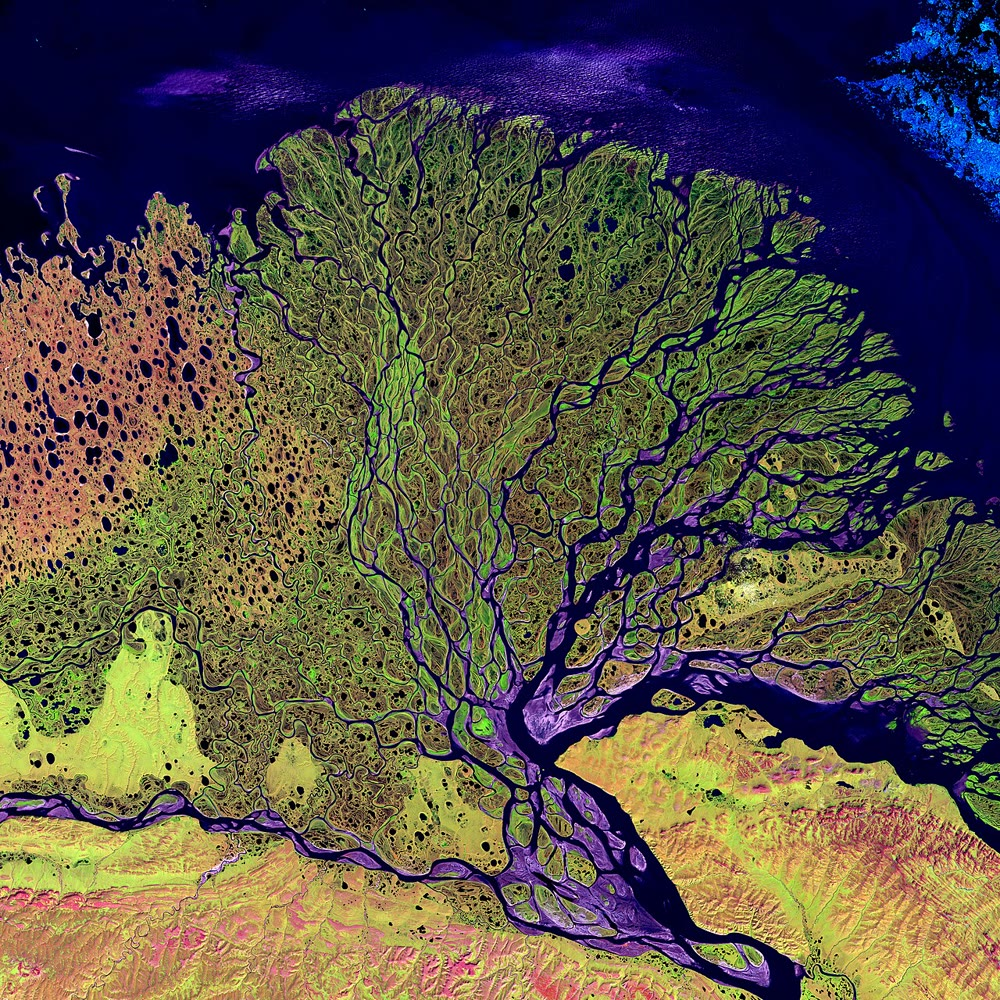
\includegraphics[width=\linewidth]{images/book1/g9-lena-delta.jpg}
\end{minipage}\hfill
\begin{minipage}[c]{0.46\linewidth}\raggedright
{\small 勒拿河\omterm{def:g5:water-shapes-the-land:delta}{三角洲}，位于西伯利亚，河水在此汇入北
冰洋：2000 年 2 月 27 日的 Landsat 假彩色图像，由短波
红外、红外和红光合成。\omterm{def:g1:landscapes-around-us:water}{河流}的众多河道
以蓝色显示。USGS EROS Data Center，经 NASA Visible Earth（公有领域，
经维基共享资源）。}
\end{minipage}
% ledger: commons:lena-landsat
\label{fig:g9:maps-of-the-earth:lena}
\end{omfigure}

\section{卫星定位}

手机或汽车能知道自己的位置，误差在几米以内，几乎
在地球上任何地方都能做到。它并不看卫星，而是接收卫星发出的信号。

\begin{definition}[卫星定位]\label{def:g9:maps-of-the-earth:positioning}
\emph{卫星定位}\index{卫星定位}是根据到
几颗位置已知的卫星的距离，确定地球上的
位置。接收机根据卫星信号
到达自身所用的时间，计算出每段距离。
\end{definition}

美国 GPS 系统始终保持至少 24 颗正常工作的卫星，
轨道高度约为 \qty{20200}{km}。每颗卫星每天绕地球两圈，分布在
环绕地球的六条轨道上，使得地球上几乎任何一点都至少能看到
四颗卫星。在 \qty{20200}{km} 外发出的信号，
以光速传播，经过 $20\,200 \div
300\,000 \approx 0.067$~s 到达。接收机测量这段时间，并将其换算为
距离。
% ledger: gps:constellation, const:c (travel time computed in figdata/grade-9/trilateration.py)

距离如何确定位置？可以在平面\omterm{def:g2:drawing-to-map:map}{地图}上设想这一思路。若接收机
距信标 A 为 \qty{5}{km}，则它位于以 A 为圆心、半径为 \qty{5}{km} 的圆上。
若它又距 B 为 \qty{10}{km}，则它同时位于两圆上，
即两圆相交的两点之一。第三个距离，
即距 C 为 \qty{5}{km}，由此选出正确的那一点。在空间中，圆变为
球面，同样的道理，还需要再多一颗卫星。

\begin{omfigure}
\begin{minipage}[c]{0.5\linewidth}\centering
\begin{tikzpicture}
\begin{axis}[x=0.42cm, y=0.42cm, xmin=-1, xmax=13, ymin=-1.5, ymax=13,
  ticks=none, axis line style={black!40}]
  \addplot[omSea!70!black, line width=0.6pt] table {figdata/out/grade-9-trilateration-circles.dat};
  \addplot[only marks, mark=triangle*, mark size=2.6pt, point meta=explicit symbolic]
    table[meta=label] {figdata/out/grade-9-trilateration-beacons.dat};
  \node[font=\footnotesize\bfseries, anchor=south west, inner sep=1pt] at (axis cs:1,7) {A};
  \node[font=\footnotesize\bfseries, anchor=south west, inner sep=1pt] at (axis cs:12,9) {B};
  \node[font=\footnotesize\bfseries, anchor=south west, inner sep=1pt] at (axis cs:9,3) {C};
  % labels first (on a white patch), then the points on top of them
  \addplot[only marks, mark=none, point meta=explicit symbolic, skip coords between index={1}{2}, opacity=0, forget plot]
    table[meta=label] {figdata/out/grade-9-trilateration-points.dat};
  \node[font=\footnotesize\bfseries, anchor=north east, xshift=-1pt, yshift=-1pt, inner sep=1pt, fill=white, text=red!75!black] at (axis cs:4,3) {R};
  \node[font=\footnotesize\bfseries, anchor=north east, xshift=-1pt, yshift=-1pt, inner sep=1pt, fill=white, text=red!75!black] at (axis cs:2.4,11.8) {F};
  \addplot[only marks, mark=none, point meta=explicit symbolic, skip coords between index={0}{1}, opacity=0, forget plot]
    table[meta=label] {figdata/out/grade-9-trilateration-points.dat};
  \node[font=\footnotesize, anchor=south west, xshift=1pt, yshift=1pt, inner sep=1pt, fill=white] at (axis cs:4,3) {R};
  \node[font=\footnotesize, anchor=south west, xshift=1pt, yshift=1pt, inner sep=1pt, fill=white] at (axis cs:2.4,11.8) {F};
  \addplot[only marks, mark=*, mark size=2pt, red!75!black, skip coords between index={1}{2}] table {figdata/out/grade-9-trilateration-points.dat};
  \addplot[only marks, mark=o, mark size=2pt, fill=white, skip coords between index={0}{1}] table {figdata/out/grade-9-trilateration-points.dat};
\end{axis}
\end{tikzpicture}
\end{minipage}\hfill
\begin{minipage}[c]{0.46\linewidth}\raggedright
{\small 平面\omterm{def:g2:drawing-to-map:map}{地图}上的定位（示意图；图中未画出以千米为单位的网格）。
接收机 R 距 A 为 \qty{5}{km}，距 B 为 \qty{10}{km}，
距 C 为 \qty{5}{km}。以 A、B 为圆心的两圆相交于 R 和一个假交点 F，只有
R 还位于以 C 为圆心的圆上。}
\end{minipage}
% ledger: (invented region: exercise data, figdata/grade-9/trilateration.py)
\label{fig:g9:maps-of-the-earth:trilateration}
\end{omfigure}

\begin{omfigure}
\begin{minipage}[t]{0.48\linewidth}\centering
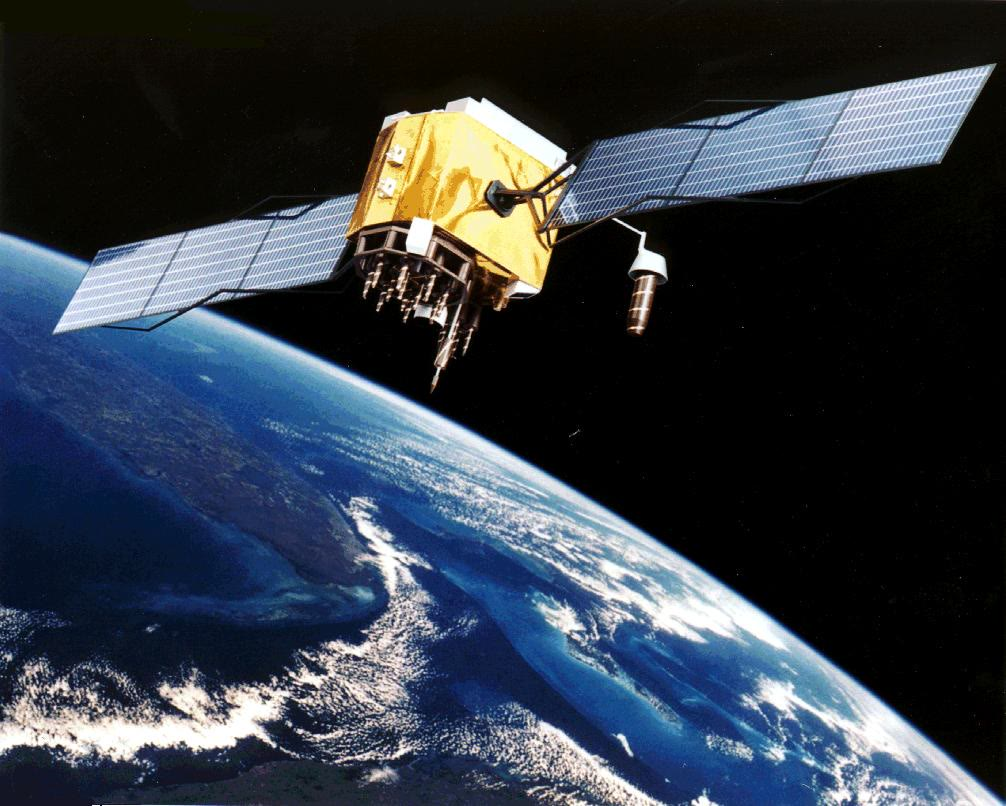
\includegraphics[width=\linewidth]{images/book1/g9-gps-satellite.jpg}

{\small 轨道中的 GPS 卫星，艺术家想象图。NASA（
公有领域，经由维基共享资源）。}
\end{minipage}\hfill
\begin{minipage}[t]{0.48\linewidth}\centering
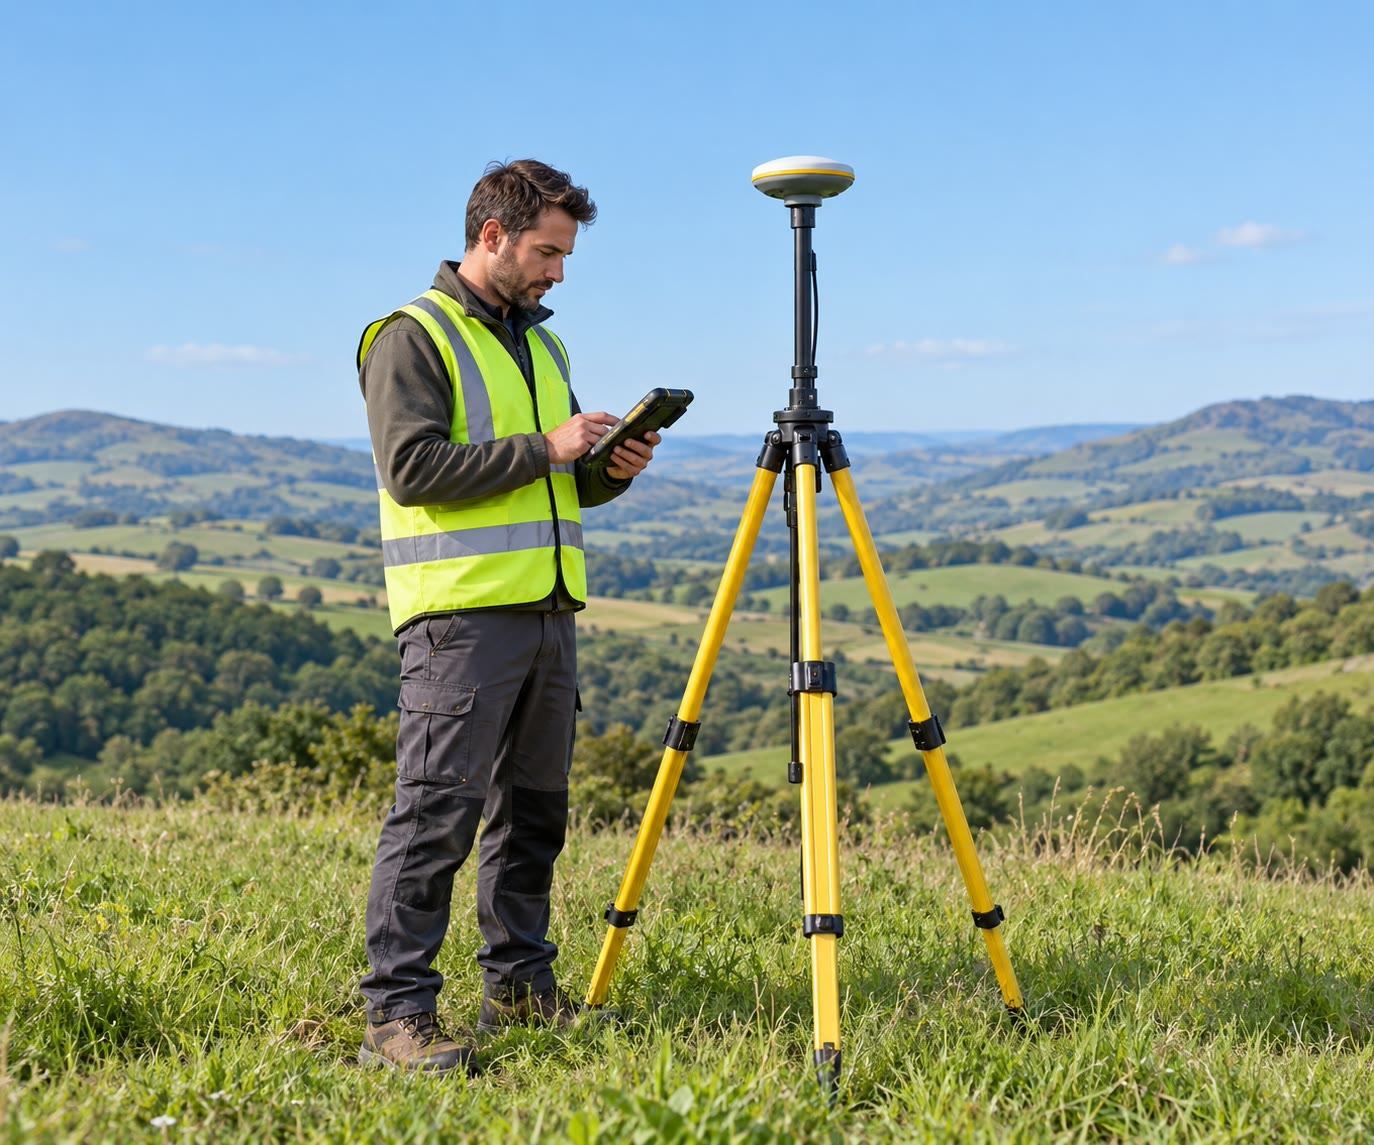
\includegraphics[width=\linewidth]{images/book1/ai/g9-surveyor.jpg}

{\small 测量员在三脚架上用卫星接收机
确定一个点的位置（插图）。}
\end{minipage}
% ledger: commons:gps-iif
\label{fig:g9:maps-of-the-earth:gps}
\end{omfigure}

\section{练习}

\begin{exercise}[$\star$]\label{exo:g9:maps-of-the-earth:1}
给出下列各描述对应的词语。(a) 将地球上每一点
对应到平面\omterm{def:g2:drawing-to-map:map}{地图}上某一点的规则。(b) 连接\omterm{def:g4:world-physical-map:altitude}{海拔}相同各点的线。
(c) 形如 $1 : 50\,000$ 的\omterm{def:g2:drawing-to-map:scale}{比例尺}。(d) 相邻两条\omterm{def:g9:maps-of-the-earth:contour}{等高线}之间的
\omterm{def:g4:world-physical-map:altitude}{海拔}差。(e) 从远处观察地球，
例如从卫星上观察。
\end{exercise}

\begin{exercise}[$\star$]\label{exo:g9:maps-of-the-earth:2}
将每段图距换算为地面实际距离，单位用米或
千米。(a) \omterm{def:g2:drawing-to-map:scale}{比例尺}为 $1 : 25\,000$ 的\omterm{def:g2:drawing-to-map:map}{地图}上 \qty{4}{cm}；(b) \omterm{def:g2:drawing-to-map:scale}{比例尺}为
$1 : 50\,000$ 的\omterm{def:g2:drawing-to-map:map}{地图}上 \qty{3}{cm}；(c) \omterm{def:g2:drawing-to-map:scale}{比例尺}为 $1 : 1\,000\,000$ 的\omterm{def:g2:drawing-to-map:map}{地图}上
\qty{2.5}{cm}；(d) 在 $1 : 25\,000$ 的\omterm{def:g2:drawing-to-map:map}{地图}上，\qty{1}{km} 对应多少厘米？
\end{exercise}

\begin{exercise}[$\star$]\label{exo:g9:maps-of-the-earth:3}
判断下列说法是否正确，并改正错误的句子。(a) \omterm{def:g3:continents-and-oceans:world-map}{世界地图}可以在不产生
任何变形的情况下完整显示整个地球。(b) 在\omterm{def:g9:maps-of-the-earth:projection}{墨卡托投影}\omterm{def:g2:drawing-to-map:map}{地图}上，格陵兰
看起来比实际更大。(c) 在\omterm{def:g9:maps-of-the-earth:projection}{等积投影}\omterm{def:g2:drawing-to-map:map}{地图}上，形状
处处都保持不变。(d) \omterm{def:g9:maps-of-the-earth:numerical-scale}{线段比例尺}在\omterm{def:g2:drawing-to-map:map}{地图}用复印机放大后
仍然正确。
\end{exercise}

\begin{exercise}[$\star$]\label{exo:g9:maps-of-the-earth:4}
在\omterm{def:g9:maps-of-the-earth:topographic-map}{地形图}上，(a) \omterm{def:g9:maps-of-the-earth:contour}{等高线}十分密集时意味着什么？
(b) \omterm{def:g9:maps-of-the-earth:contour}{等高线}十分稀疏时意味着什么？(c) 由外向内升高的闭合\omterm{def:g9:maps-of-the-earth:contour}{等高线}
表示什么？(d) 为什么两条\omterm{def:g9:maps-of-the-earth:contour}{等高线}永远不会相交？
\end{exercise}

\begin{exercise}[$\star\star$]\label{exo:g9:maps-of-the-earth:5}
% ledger: data:ne-land (factor 1/cos^2, figdata/grade-9/projections.py)
在\omterm{def:g9:maps-of-the-earth:projection}{墨卡托投影}\omterm{def:g2:drawing-to-map:map}{地图}上，与\omterm{def:g3:continents-and-oceans:equator}{赤道}相比，\omterm{def:g6:latitude-longitude:latitude}{纬度} \ang{60} 处的面积放大 4 倍，\omterm{def:g6:latitude-longitude:latitude}{纬度}
\ang{30} 处约放大 1.33 倍。(a) \omterm{def:g2:drawing-to-map:map}{地图}上画出了一个面积为
\qty{1000}{km^2}、位于北纬 \ang{60} 的\omterm{def:g1:landscapes-around-us:water}{湖泊}。若位于\omterm{def:g3:continents-and-oceans:equator}{赤道}的\omterm{def:g1:landscapes-around-us:water}{湖泊}在\omterm{def:g2:drawing-to-map:map}{地图}上画成相同大小，
其实际面积为多少？(b) 两个实际面积相同的岛屿，
分别位于 \ang{30} 与 \ang{60}。第二个在\omterm{def:g2:drawing-to-map:map}{地图}上
看起来是第一个的多少倍？(c) 为什么\omterm{def:g9:maps-of-the-earth:projection}{墨卡托投影}\omterm{def:g2:drawing-to-map:map}{地图}永远无法
显示两极？
\end{exercise}

\begin{exercise}[$\star\star$]\label{exo:g9:maps-of-the-earth:6}
% ledger: (invented region: the Varden Hills map of the chapter)
利用本章中瓦尔登\omterm{def:g1:landscapes-around-us:landform}{丘陵}的\omterm{def:g9:maps-of-the-earth:topographic-map}{地形图}。(a) \omterm{def:g9:maps-of-the-earth:contour}{等高距}是多少？
(b) 图中以高程点标注的山顶\omterm{def:g4:world-physical-map:altitude}{海拔}是多少，
及紧靠其周围的计曲线\omterm{def:g4:world-physical-map:altitude}{海拔}是多少？(c) \omterm{def:g1:landscapes-around-us:water}{河流}向东流，
图中谷底在西部还是东部更高？
(d) 沿 C--D，在\omterm{def:g1:landscapes-around-us:water}{河流}以北，哪两条\omterm{def:g9:maps-of-the-earth:contour}{等高线}之间
最为密集？这说明该处坡度如何？
\end{exercise}

\begin{exercise}[$\star\star$]\label{exo:g9:maps-of-the-earth:7}
% ledger: (invented region: profile C--D, figdata/grade-9/varden_topo.py)
利用本章中的剖面 C--D。(a) C
和 D 大约位于什么\omterm{def:g4:world-physical-map:altitude}{海拔}？(b) 沿剖面的最低\omterm{def:g4:world-physical-map:altitude}{海拔}是多少，
该点离 C 多远？(c) 沿 C--D 的平坦谷底有多长？(d) 剖面图
的竖直比例放大了三倍。
制图者为何常这样做？
\end{exercise}

\begin{exercise}[$\star\star$]\label{exo:g9:maps-of-the-earth:8}
在 $1 : 25\,000$ 的\omterm{def:g2:drawing-to-map:map}{地图}上，一条小路穿过 \qty{200}{m} \omterm{def:g9:maps-of-the-earth:contour}{等高线}后，
再穿过 \qty{300}{m} \omterm{def:g9:maps-of-the-earth:contour}{等高线}，两交点在图上相距 \qty{2}{cm}。(a) 两点
在地面上的水平距离是多少？(b) 这段路
爬升了多少？(c) 坡度是多少？用百分数表示。(d) 再往前，
两条\omterm{def:g4:world-physical-map:altitude}{海拔}相差 \qty{100}{m} 的\omterm{def:g9:maps-of-the-earth:contour}{等高线}，在图上相距 \qty{4}{cm}。
这段路比前面更陡还是更缓？相差多少？
\end{exercise}

\begin{exercise}[$\star\star$]\label{exo:g9:maps-of-the-earth:9}
% ledger: usgs:landsat1
Landsat~1 号每天绕地球 14 圈，每 18 天
经过同一地点。(a) 两次经过同一地点之间，它绕行了多少圈？
(b) 每圈用时 103 分钟。14 圈共需多少
小时？(c) 它设计工作一年，在发射五年半后的
1978 年 1 月 6 日关机。它实际工作的时间
是设计寿命的多少倍？(d) 请举出一项地表变化，
同一地点相隔数年拍摄的影像可以显示这种变化。
\end{exercise}

\begin{exercise}[$\star\star$]\label{exo:g9:maps-of-the-earth:10}
% ledger: gps:constellation, const:c
一颗 GPS 卫星距离约 \qty{20200}{km}，其信号
以约每秒 \qty{300000}{km} 的速度传播。(a) 信号
到达需要多长时间？答案用科学记数法表示。(b) 若接收机的
时钟误差为 $1 \times 10^{-3}$~s，会造成多大的
距离误差？(c) 这说明\omterm{def:g9:maps-of-the-earth:positioning}{卫星定位}所用的时钟
应具备怎样的要求？
\end{exercise}

\begin{exercise}[$\star\star\star$]\label{exo:g9:maps-of-the-earth:11}
在一张以千米为单位的方格\omterm{def:g2:drawing-to-map:plan}{平面图}上，信标 A 位于 $(0, 0)$，
信标 B 位于 $(10, 0)$，接收机与 A 相距 \qty{6}{km}，与 B 相距
\qty{8}{km}。(a) 证明点 $(3.6, 4.8)$ 与 A 相距 \qty{6}{km}，
与 B 相距 \qty{8}{km}。(b) 再给出一个与 A、B 距离相同的点。
(c) 第三个信标 C 位于 $(0, 10)$，接收机与 C 相距
约 \qty{6.3}{km}。两点中哪一点是接收机？(d) \omterm{def:g9:maps-of-the-earth:positioning}{卫星定位}
为什么需要多颗卫星？
\end{exercise}

\begin{exercise}[$\star\star\star$]\label{exo:g9:maps-of-the-earth:12}
% ledger: data:ne-land (areas, figdata/grade-9/projections.py)
非洲\omterm{def:g3:continents-and-oceans:continent}{大陆}面积约为 2900 万 \unit{km^2}，格陵兰岛约为
210 万 \unit{km^2}。(a) 非洲面积是格陵兰岛的多少倍？(b)
在墨卡托\omterm{def:g2:drawing-to-map:map}{地图}上，格陵兰岛中部附近（约北纬 \ang{72}）的面积被放大约
10.5 倍。估算格陵兰岛在该\omterm{def:g2:drawing-to-map:map}{地图}上呈现的面积。
(c) 非洲横跨\omterm{def:g3:continents-and-oceans:equator}{赤道}，\omterm{def:g3:continents-and-oceans:equator}{赤道}附近的面积放大很小。
将 (b) 的结果与非洲面积比较，并解释本章开头的
那幅挂图为何如此。(d) 你会选择哪种投影来公平地
显示各\omterm{def:g3:continents-and-oceans:continent}{大陆}的大小？
\end{exercise}

\section{问题：穿越瓦尔登丘陵的小路}

\begin{problem}[{周末问题——规划者在地形图上画出了一条穿越
瓦尔登丘陵的小路；最终答案为小路的长度（以千米计）及其
总爬升（以米计）}]
\label{pb:g9:maps-of-the-earth:1}
% ledger: (invented region: the Varden Hills, figdata/grade-9/varden_topo.py, part problem: leg lengths 3.6 / 2.5 / 2.35 cm, spot heights 296 / 143 / 335 / 544 m, 4.2 km, 401 m)
小路从农场 S 出发，下行至河上的桥 B，
再爬升至小屋 W，最后到达山顶 T。每一段都是直线，
且只下行或只上行。\omterm{def:g2:drawing-to-map:map}{地图}\omterm{def:g2:drawing-to-map:scale}{比例尺}为 $1 : 50\,000$；
S、B、W、T 各点的\omterm{def:g4:world-physical-map:altitude}{海拔}标注在其旁边。

\begin{omfigure}
\begin{tikzpicture}
\begin{axis}[x=1.6cm, y=1.6cm, xmin=2, xmax=8, ymin=1.8, ymax=6.2, ticks=none,
  axis line style={black!60}, clip mode=individual]
  \addplot[contour] table {figdata/out/shared-region-contours.dat};
  \addplot[index contour] table {figdata/out/shared-region-index-contours.dat};
  \addplot[river] table {figdata/out/shared-region-river.dat};
  \addplot[only marks, mark=none, point meta=explicit symbolic, nodes near coords,
    nodes near coords align={center}, nodes near coords style={font=\tiny, fill=white, inner sep=0.6pt, text=omContour}]
    table[meta=label] {figdata/out/grade-9-varden_topo-labels.dat};
  \addplot[red!75!black, line width=1pt, dashed] table[x=x_km, y=y_km] {figdata/out/grade-9-varden_topo-path.dat};
  \addplot[only marks, mark=*, mark size=1.6pt, red!75!black, point meta=explicit symbolic, nodes near coords align={right}]
    table[meta=label] {figdata/out/grade-9-varden_topo-points.dat};
  \node[red!75!black, font=\scriptsize\bfseries, text=black, fill=white, fill opacity=0.8, text opacity=1, inner sep=1pt, anchor=south] at (axis cs:2.9,2.3) {S\,(296)};
  \node[red!75!black, font=\scriptsize\bfseries, text=black, fill=white, fill opacity=0.8, text opacity=1, inner sep=1pt, anchor=south] at (axis cs:3.8,3.84) {B\,(143)};
  \node[red!75!black, font=\scriptsize\bfseries, text=black, fill=white, fill opacity=0.8, text opacity=1, inner sep=1pt, anchor=south] at (axis cs:4.6,4.8) {W\,(335)};
  \node[red!75!black, font=\scriptsize\bfseries, text=black, fill=white, fill opacity=0.8, text opacity=1, inner sep=1pt, anchor=south] at (axis cs:5.38,5.68) {T\,(544)};
  \coordinate (na) at (axis cs:8.35,5.4);
\end{axis}
\pic at (na) {northarrow};
\end{tikzpicture}

{\small 瓦尔登\omterm{def:g1:landscapes-around-us:landform}{丘陵}\omterm{def:g9:maps-of-the-earth:topographic-map}{地形图}上的小路 S--B--W--T
（此处为缩小图；原图\omterm{def:g2:drawing-to-map:scale}{比例尺}为 $1 : 50\,000$，各段长度
分别为 3.6、2.5 和 \qty{2.35}{cm}）。}
\label{fig:g9:maps-of-the-earth:path}
\end{omfigure}

\noindent\textbf{第一部分——\omterm{def:g2:drawing-to-map:map}{地图}上的路线。}\par\nopagebreak
\begin{enumerate}[beginpenalty=10000]
  \item \omterm{def:g2:drawing-to-map:scale}{比例尺}为 $1 : 50\,000$ 时，\omterm{def:g2:drawing-to-map:map}{地图}上 \qty{1}{cm}
        代表地面上多少米？
  \item 在原图上，S--B 段长 \qty{3.6}{cm}。它在地面上的
        长度为多少千米？
  \item B--W 段和 W--T 段分别长 \qty{2.5}{cm} 和 \qty{2.35}{cm}。
        它们在地面上各长多少？
  \item 从 B 到 T，小路大致朝哪个方向延伸？
\end{enumerate}

\noindent\textbf{第二部分——爬升。}\par\nopagebreak
\begin{enumerate}[resume, beginpenalty=10000]
  \item \omterm{def:g2:drawing-to-map:map}{地图}的\omterm{def:g9:maps-of-the-earth:contour}{等高距}是多少？
  \item 哪一段是下行的？下降了多少米？
  \item B--W 段和 W--T 段分别爬升了多少米？
  \item W--T 段的平均坡度是多少？用百分数表示。
  \item 规划者为何没有把小路画成从 S
        直达 T 的直线？
\end{enumerate}

\noindent\textbf{第三部分——步行。}\par\nopagebreak
\begin{enumerate}[resume, beginpenalty=10000]
  \item 设某人在平路上每小时走 \qty{4}{km}，每爬升
        \qty{10}{m} 需多花一分钟。整段步行
        需要多长时间？
  \item 另一人沿小路反向行走，从 T 到 S。
        她爬升了多少米？
  \item 小路的总长度是多少千米，及其
        总爬升是多少米？
\end{enumerate}
\end{problem}
